\documentclass{article}
\usepackage[utf8]{inputenc}
\usepackage{graphicx}
\usepackage{titling}
\usepackage{titlesec}
\usepackage{booktabs}
\usepackage{fancyhdr}
\usepackage{lipsum}
\usepackage{comment}
\usepackage{enumitem}
\usepackage{listings}
\usepackage{xcolor}
\usepackage{longtable}
\usepackage{cite}


\lstdefinestyle{pidstyle}{
    basicstyle=\ttfamily\footnotesize,
    breaklines=true,
    escapechar=\#, % Define escape character for inline LaTeX commands
    linewidth=\textwidth,
    basicstyle=\ttfamily\scriptsize
}

\renewcommand{\maketitle}{%
  \begin{leftmark}
    \vspace*{\baselineskip} % Add a bit of vertical space

%    \includegraphics[width=4cm]{example-image-a} % Add an image before the title. you will need to replace the image path with your own

%    \vspace{0.5cm} % Add vertical space before title

    \textbf{\fontsize{18}{36}\selectfont \thetitle} % Font Size and Bold Title

     \vspace{0.05cm} % Add vertical space before subtitle
%    \textit{\Large \theauthor}  % Subtitle / Author
    \vspace{\baselineskip} % Add vertical space after subtitle
     \rule{\textwidth}{0.4pt} % Add a horizontal line

   \end{leftmark}
%    \thispagestyle{empty} % Prevent header/footer on the title page
}


% Section Formatting
\titleformat{\section}
  {\normalfont\fontsize{18}{22}\bfseries} % Font and style
  {\thesection}         % Section number
  {1em}                   % Horizontal space after section number
  {}                     % Code before the section name
  []                     % Code after the section name

\titleformat{\subsection}
  {\normalfont\fontsize{14}{18}\bfseries} % Font and style
  {\thesubsection}         % Subsection number
  {1em}                   % Horizontal space after subsection number
  {}                     % Code before the subsection name
  []                     % Code after the subsection name

\setlength{\parindent}{0pt}

\title{Computing platforms (Spring 2025)\newline
week 1}
\author{Juha-Pekka Heikkilä}



\pagestyle{fancy}
\fancyhf{}

\renewcommand{\headrulewidth}{0pt}

\newcommand{\footerline}{\makebox[\textwidth]{\hrulefill}}

\newcommand{\footercontent}{%
    \begin{tabular}{@{}l@{}}
        \footerline \\
        \leftmark \hfill \rlap{\thepage}
    \end{tabular}
}

\fancyfoot[C]{\footercontent}


\newcommand{\exercise}[1]{
    \section*{Exercise #1}
    \markboth{Exercise #1}{}
}



\begin{document}
\maketitle


\exercise{1}
Pick an operating system of your choice and answer the following questions.
\begin{enumerate}[label=\textbf{\alph*})]
    \item MacOS
    \item   CLI program on MacOS to monitor running programs is {\bf ps}.
    System level API for same information is found in {\bf sysctl} call.
    \item Let's select running VSCode app for inspection (PID 5112 below):

    \begin{lstlisting}[
        style=pidstyle
    ]
    $ ps|grep -i "Visual Studio Code.app"
    #\textcolor{black}{34048}# ttys008    0:00.01 grep -i Visual Studio Code.app
    #\textcolor{red}{5112}#  ttys011    0:00.02 /opt/homebrew/bin/bash --init-file /Applications/Visual Studio Code.app/Contents/Resources/app/out/vs/workbench/contrib/terminal/common/scripts/shellIntegration-bash.sh
    \end{lstlisting}

    We can get all the essential information using command:
    \begin{lstlisting}[
        style=pidstyle
    ]
        ps -p 5112 -o pid,ppid,uid,user,%cpu,%mem,vsz,rss,tty,stat,start,time,command
    \end{lstlisting}
    which give
    \begin{lstlisting}[
        style=pidstyle,
        xleftmargin=-1cm,
        framexleftmargin=-1cm
    ]
        PID  PPID   UID USER  %CPU %MEM      VSZ    RSS TTY      STAT STARTED      TIME COMMAND
        5112  5097   501 juha   0,0  0,0 410296320    208 ttys011  Ss+  11Tam25   0:00.02 /opt/homebrew/bin/bash --init-file /Applications/Visual Studio Code.app/Contents/Resources/app/out/vs/workbench/contrib/terminal/common/scripts/shellIntegration-bash.sh
    \end{lstlisting}

    Legend for above listed process information:
    {\ttfamily\scriptsize
    \begin{longtable}{|l|p{12cm}|}
        \hline
        \textbf{Parameter} & \textbf{Description} \\ \hline
        PID & Process ID, a unique identifier for the process. \\ \hline
        PPID & Parent Process ID, the ID of the process that started this process. \\ \hline
        UID & User ID, the numerical identifier of the process owner. \\ \hline
        USER & Username of the process owner. \\ \hline
        \%CPU & Percentage of CPU being used by the process. \\ \hline
        \%MEM & Percentage of memory being used by the process. \\ \hline
        VSZ & Virtual memory size used by the process, in kilobytes. \\ \hline
        RSS & Resident Set Size, the amount of physical memory used by the process, in kilobytes. \\ \hline
        TTY & The terminal associated with the process. \\ \hline
        STAT & Current status of the process (e.g., \texttt{S} for sleeping, \texttt{R} for running). \\ \hline
        STARTED & The time or date when the process started. \\ \hline
        TIME & Cumulative CPU time used by the process (in the format \texttt{HH:MM:SS}). \\ \hline
        COMMAND & The full command with arguments that was used to start the process. \\ \hline
        \end{longtable}
    }


\end{enumerate}


\newpage
\exercise{2}
Process creation and termination.
\begin{enumerate}[label=\textbf{\alph*})]
    \item
    \textbf{Briefly describe what happens when a process is created?}

    Process creation involves several well defined steps to prepare a new
    process for execution. According to Stallings\cite{stallings}, the general
    steps for process creation are as follows:
    
    \begin{enumerate}[label=\textbf{\arabic*.}]
        \item \textbf{Assign a unique identifier:} Each created process is given an unique
        identifier. This is added to the process table, which has an entry for each process.
    
        \item \textbf{Allocate space:} Memory is allocated for the process'es image,
        including program, data, and stack. If the process inherit memory or
        resources from a parent process, the appropriate linkages are set up.
    
        \item \textbf{Initialize process control block content:}
        \begin{itemize}
            \item Identification portion, contain such as PID and parent PID.
            \item Processor state, being mostly zero except for program counter and stack pointers.
            \item Control information, such as the initial state
            (Ready or Ready/Suspend) and priority.
        \end{itemize}
    
        \item \textbf{Set scheduling linkages:} The process is added to
        appropriate scheduling queue such as the Ready queue or Ready/Suspend queue.
    
        \item \textbf{Create or expand other data structures:} Accounting files and
        other structures are initialized for monitoring, billing, or performance evaluation.
    \end{enumerate}
        

    \pagebreak
    \item
    \textbf{List and describe three different reasons leading to process termination}

    Processes in an operating system can terminate for various reasons.
    Below are three common causes, along with their descriptions and examples in MacOS:

\begin{enumerate}[label=\textbf{\arabic*.}]
    \item \textbf{Normal Completion}
    \begin{itemize}
        \item \textbf{Description:} A process terminates normally when
        it successfully completes the execution of its program.
        \item \textbf{Example:} In MacOS, a process calls the \texttt{exit()}
        system call to signal successful completion. The operating system cleans
        up resources and notifies the parent process.
    \end{itemize}

    \item \textbf{Error or Exception}
    \begin{itemize}
        \item \textbf{Description:} Processes terminate abnormally due to
        runtime errors or exceptions such as division by zero or segmentation faults.
        \item \textbf{Example:} In MacOS, dereferencing a null pointer results
        in a segmentation fault terminating the process.
    \end{itemize}

    \item \textbf{External Termination (Kill or Signal)}
    \begin{itemize}
        \item \textbf{Description:} A process is terminated by an external factor, such as:
        \begin{itemize}
            \item A parent process sending a termination signal (\texttt{SIGKILL}, \texttt{SIGTERM}).
            \item System-initiated termination during shutdown or when resources are insufficient (For example OOM-killer).
        \end{itemize}
        \item \textbf{Example:} Using the \texttt{kill} command to send a \texttt{SIGKILL} signal:
        \begin{lstlisting}[
            style=pidstyle
        ]
        kill -9 <PID>
        \end{lstlisting}
    \end{itemize}
\end{enumerate}
\end{enumerate}





\newpage
\exercise{3}

\textbf{Context switch on the TOY processor.}

\begin{enumerate}[label=\textbf{\alph*})]
    \item \textbf{What information about the context of a process needs to be saved to the process control block (PCB) during a mode switch?}
    
    When a mode switch occurs, the operating system must save the current context of the process to its PCB to ensure it can resume execution later. The following information is saved:
    \begin{itemize}
        \item General-purpose registers R0 .. R3: These contain the current working
        data of the process.
        \item Special registers:
        \begin{itemize}
            \item SP (Stack Pointer): Tracks the top of the user process's stack.
            \item FP (Frame Pointer): Tracks the base of the current stack frame.
            \item PC (Program Counter): Indicates the next instruction to be executed.
        \end{itemize}
        \item Process priority, execution state, and any information required
        for scheduling or resource management.
    \end{itemize}


    \item \textbf{What happens during a mode switch when an interrupt occurs?}

    When an interrupt occurs, the TOY processor performs the following steps:
    \begin{enumerate}
        \item Save the Program Counter (PC): The address of the next instruction
        in the user process is saved to the \textbf{EPC} register.
        \item Load Interrupt Handler Address: Address of interrupt
        handler is loaded into the \textbf{PC} register, switching execution
        to interrupt handler.
        \item Switch to System Mode: Processor changes its mode from user to system,
        enabling access to all registers, including \textbf{K0} and \textbf{K1}.
        \item Execute Interrupt Handler: Processor begin executing
        instructions from interrupt handler.
    \end{enumerate}

    \item \textbf{What happens during a mode switch when the operating system returns to the interrupted process?}

    After interrupt is handled operating system restores the context of
    interrupted process:
    \begin{enumerate}
        \item Restore PC: Address saved in the \textbf{EPC} register in part b
        is copied back to the \textbf{PC} register.
        \item Switch to User Mode: Processor changes mode from system to user, restricting access to \textbf{EPC}, \textbf{K0}, and \textbf{K1}.
        \item Resume Execution: Process continues execution from  address now stored in the \textbf{PC} register, resuming where it was interrupted.
    \end{enumerate}
\end{enumerate}

\newpage
\exercise{4}
\textbf{Processes and process states.}

\begin{enumerate}[label=\textbf{\alph*})]
    \item \textbf{process-run.py execution}
    \begin{figure}[ht]
        \centering
        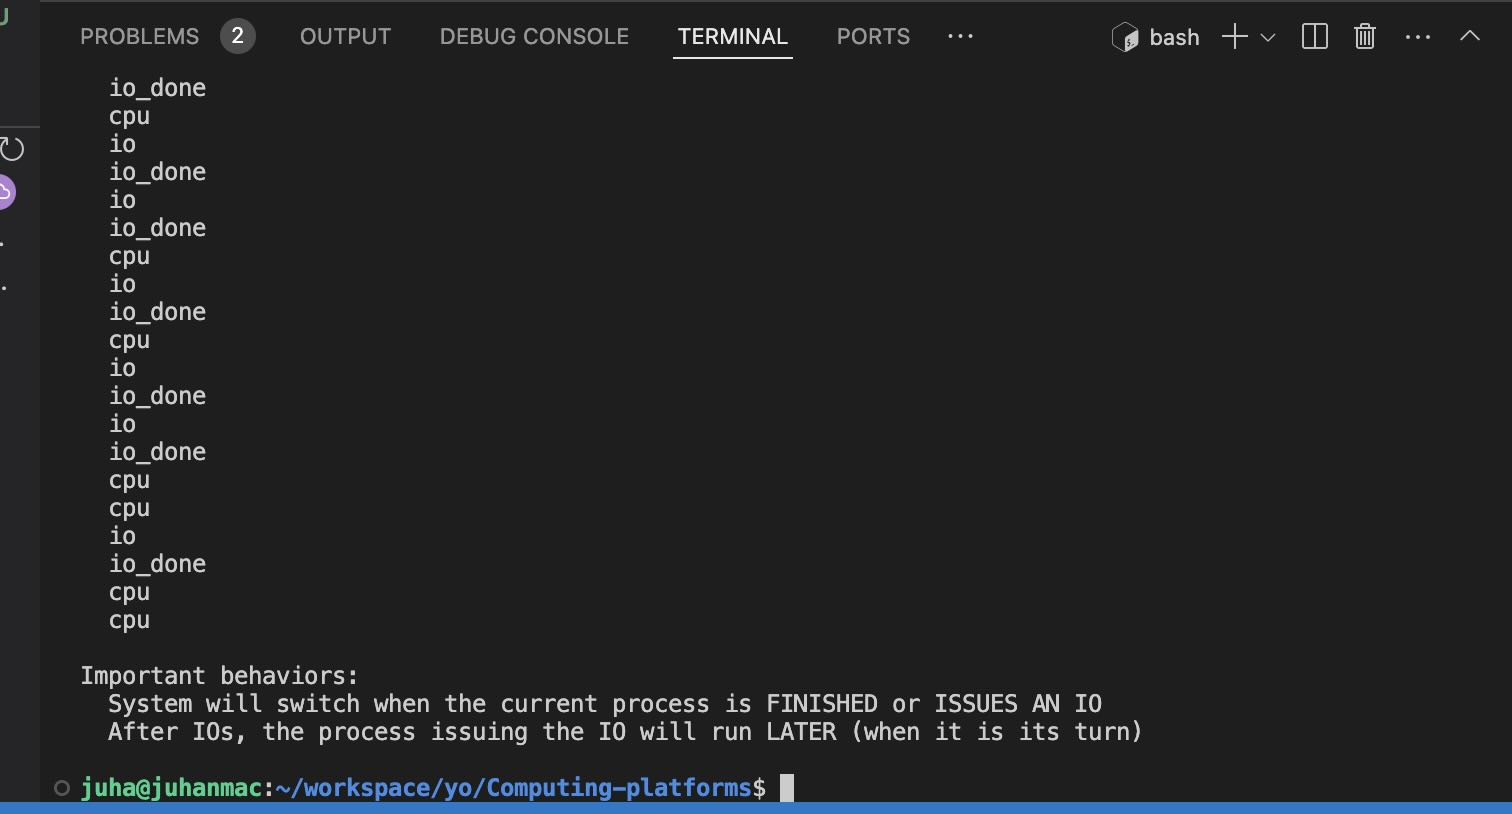
\includegraphics[width=\textwidth]{process-run-py.jpg}
        \caption{Process Execution Diagram}
        \label{fig:process-run-py}
    \end{figure}
    \item \textbf{cpu-intro.pdf questions 1, 2}

    \begin{enumerate}[label=\textbf{\arabic*}), start=1]
        \item
        {\bf Run process-run.py with the following flags:
        -l 5:100,5:100. What should the CPU utilization be}

        100\% because flags say cpu utilization is 100\%
        \item
        {\bf Now run with these flags: ./process-run.py
        -l 4:100,1:0.}

        As it's seen in results, second PID get to execute
        after first PID and will be blocked while IO is in
        progress. Both processes complete after 11 cycles.

        {\scriptsize
        \begin{verbatim}
$ python3 ./process-run.py -l 4:100,1:0 -c -p
Time        PID: 0        PID: 1           CPU           IOs
  1        RUN:cpu         READY             1          
  2        RUN:cpu         READY             1          
  3        RUN:cpu         READY             1          
  4        RUN:cpu         READY             1          
  5           DONE        RUN:io             1          
  6           DONE       BLOCKED                           1
  7           DONE       BLOCKED                           1
  8           DONE       BLOCKED                           1
  9           DONE       BLOCKED                           1
 10           DONE       BLOCKED                           1
 11*          DONE   RUN:io_done             1          

Stats: Total Time 11
Stats: CPU Busy 6 (54.55%)
Stats: IO Busy  5 (45.45%)
        \end{verbatim}
        }

    \end{enumerate}
\end{enumerate}


\exercise{5}
\textbf{Processes and process states (cont’d)}

\begin{enumerate}[label=\textbf{\arabic*}), start=3]
    \item
    {\bf Switch the order of the processes: -l
    1:0,4:100. What happens now?}

    Now first PID get blocked when it start to do I/O which
    follow there's context switch to second PID which get to
    use CPU. This interleaves two processes making overall
    process faster. Now both PIDs finish in 7 cycles instead of
    previously seen 11 cycles.

    \item
    {\bf We’ll now explore some of the other flags. What happens
    when you run the following two processes (-l 1:0,4:100
    -c \linebreak -S SWITCH\_ON\_END), one doing I/O and the
    other doing CPU work?}

    Now context switching is blocked until one PID is finished,
    this cause second PID to wait until I/O on first PID is
    finished. Effect of this for final result is overall process
    take 11 cycles, e.g. same as seen in {\bf 2)}.

    \item
    {\bf Now, run the same processes, but with the switching
    behavior set to switch to another process whenever one
    is WAITING for I/O (-l 1:0,4:100 -c -S SWITCH\_ON\_IO).
    What happens now?}

    Now we see same result as on {\bf 3)}, ie. while PID become
    blocked by I/O another PID will be switched on to.
\pagebreak
    \item 
    {\bf  One other important behavior is what to do when
    an I/O completes. What happens when you run this combination
    of processes? (./process-run.py -l 3:0,5:100,5:100,5:100
    -S SWITCH\_ON\_IO -c -p -I IO\_RUN\_LATER). Are system
    resources being effectively utilized?}

    No, system resources are not being effectively utilized.
    This can be seen from table below where interleaving
    CPU and I/O is not perfect:

    {\scriptsize

    \begin{verbatim}
$ python3 ./process-run.py -l 3:0,5:100,5:100,5:100 -S SWITCH_ON_IO -c -p -I IO_RUN_LATER 
Time        PID: 0        PID: 1        PID: 2        PID: 3           CPU           IOs
  1         RUN:io         READY         READY         READY             1          
  2        BLOCKED       RUN:cpu         READY         READY             1             1
  3        BLOCKED       RUN:cpu         READY         READY             1             1
  4        BLOCKED       RUN:cpu         READY         READY             1             1
  5        BLOCKED       RUN:cpu         READY         READY             1             1
  6        BLOCKED       RUN:cpu         READY         READY             1             1
  7*         READY          DONE       RUN:cpu         READY             1          
  8          READY          DONE       RUN:cpu         READY             1          
  9          READY          DONE       RUN:cpu         READY             1          
 10          READY          DONE       RUN:cpu         READY             1          
 11          READY          DONE       RUN:cpu         READY             1          
 12          READY          DONE          DONE       RUN:cpu             1          
 13          READY          DONE          DONE       RUN:cpu             1          
 14          READY          DONE          DONE       RUN:cpu             1          
 15          READY          DONE          DONE       RUN:cpu             1          
 16          READY          DONE          DONE       RUN:cpu             1          
 17    RUN:io_done          DONE          DONE          DONE             1          
 18         RUN:io          DONE          DONE          DONE             1          
 19        BLOCKED          DONE          DONE          DONE                           1
 20        BLOCKED          DONE          DONE          DONE                           1
 21        BLOCKED          DONE          DONE          DONE                           1
 22        BLOCKED          DONE          DONE          DONE                           1
 23        BLOCKED          DONE          DONE          DONE                           1
 24*   RUN:io_done          DONE          DONE          DONE             1          
 25         RUN:io          DONE          DONE          DONE             1          
 26        BLOCKED          DONE          DONE          DONE                           1
 27        BLOCKED          DONE          DONE          DONE                           1
 28        BLOCKED          DONE          DONE          DONE                           1
 29        BLOCKED          DONE          DONE          DONE                           1
 30        BLOCKED          DONE          DONE          DONE                           1
 31*   RUN:io_done          DONE          DONE          DONE             1          

Stats: Total Time 31
Stats: CPU Busy 21 (67.74%)
Stats: IO Busy  15 (48.39%)
    \end{verbatim}
    }
\pagebreak
    \item 
    {\bf Now run the same processes, but with
    -I IO\_RUN\_IMMEDIATE set, which immediately runs
    the process that issued the I/O. How does this behavior
    differ? Why might running a process that just completed
    an I/O again be a good idea?}

    Now interleaving of PIDs is well aligned which is seen at 100\% CPU
    utilization. Swtiching to process that just completed I/O maybe good
    idea if it has more I/O operations in queue. This will allow slow I/O
    operations to be running continuously.


{\scriptsize
\begin{verbatim}
$ python3 ./process-run.py -l 3:0,5:100,5:100,5:100 -S SWITCH_ON_IO -c -p -I IO_RUN_IMMEDIATE
Time        PID: 0        PID: 1        PID: 2        PID: 3           CPU           IOs
  1         RUN:io         READY         READY         READY             1          
  2        BLOCKED       RUN:cpu         READY         READY             1             1
  3        BLOCKED       RUN:cpu         READY         READY             1             1
  4        BLOCKED       RUN:cpu         READY         READY             1             1
  5        BLOCKED       RUN:cpu         READY         READY             1             1
  6        BLOCKED       RUN:cpu         READY         READY             1             1
  7*   RUN:io_done          DONE         READY         READY             1          
  8         RUN:io          DONE         READY         READY             1          
  9        BLOCKED          DONE       RUN:cpu         READY             1             1
 10        BLOCKED          DONE       RUN:cpu         READY             1             1
 11        BLOCKED          DONE       RUN:cpu         READY             1             1
 12        BLOCKED          DONE       RUN:cpu         READY             1             1
 13        BLOCKED          DONE       RUN:cpu         READY             1             1
 14*   RUN:io_done          DONE          DONE         READY             1          
 15         RUN:io          DONE          DONE         READY             1          
 16        BLOCKED          DONE          DONE       RUN:cpu             1             1
 17        BLOCKED          DONE          DONE       RUN:cpu             1             1
 18        BLOCKED          DONE          DONE       RUN:cpu             1             1
 19        BLOCKED          DONE          DONE       RUN:cpu             1             1
 20        BLOCKED          DONE          DONE       RUN:cpu             1             1
 21*   RUN:io_done          DONE          DONE          DONE             1          

Stats: Total Time 21
Stats: CPU Busy 21 (100.00%)
Stats: IO Busy  15 (71.43%)
\end{verbatim}
}
\end{enumerate}

\newpage
\bibliographystyle{plain}
\bibliography{references}
\end{document}
